\begin{figure}[h]
    \centering
    \makebox[\columnwidth][c]{
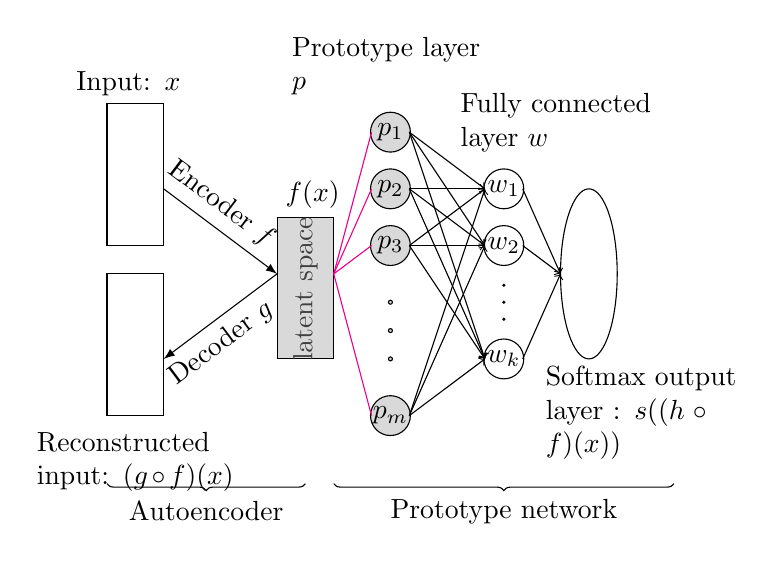
\begin{tikzpicture}[scale=0.72]
  \filldraw[fill=white, draw=black] (0,0) rectangle (1,2.5) ;
  \path (0,0) -- (1,2.5) node[midway, below,  yshift=-2.8em, text width=2.5cm] {Reconstructed input: $(g \circ f)(\bm{x})$ };
  \filldraw[fill=white, draw=black] (0,3) rectangle (1,5.5);
  \path (0,3) -- (1,5.5) node[midway, above, yshift=2.5em, text width=1.5cm] {Input: $\bm{x}$ };
;
\filldraw[fill=gray!30, draw=black] (3,1) rectangle (4,3.5);
\path (3,2) -- (4,4) node[midway, above, yshift=1em, xshift=0.75cm, text width=2cm]{ $f(\bm{x})$} node[color=darkgray,rotate=90,midway,xshift=-0.55cm] {latent space};
\path[-latex] (3, 2.5) edge node [xshift=-0.2cm, sloped, below] {Decoder $g$} (1,1) ;
\path[-latex] (1, 4) edge node [xshift=-0.2cm, sloped, above] {Encoder $f$} (3,2.5);
\coordinate (p1) at (5,0);
\coordinate (p2) at (5,2);
\coordinate (p3) at (5,3);
\coordinate (p4) at (5,4);
\coordinate (pn) at (5,5);
\coordinate (o1) at (7,1);
\coordinate (o2) at (7,2);
\coordinate (o3) at (7,3);
\coordinate (o4) at (7,4);
\filldraw[fill=gray!30, draw=black] (p1) circle (1em) node {$p_m$};
\filldraw[fill=gray!30, draw=black] (p2) circle (0.1em);
\filldraw[fill=gray!30, draw=black] (5,1.5) circle (0.1em);
\filldraw[fill=gray!30, draw=black] (5,1) circle (0.1em);
\filldraw[fill=gray!30, draw=black] (p3) circle (1em) node {$p_3$};
\filldraw[fill=gray!30, draw=black] (p4) circle (1em) node {$p_2$};
\filldraw[fill=gray!30, draw=black] (pn) circle (1em) node {$p_1$}  node[above, yshift=1em, text width=2.5cm] {Prototype layer $p$};
\filldraw[fill=white, draw=black] (o1) circle (1em) node {$w_k$};
\filldraw[fill=gray!30, draw=black] (7,2) circle (0.05em);
\filldraw[fill=gray!30, draw=black] (7,2-0.3) circle (0.05em);
\filldraw[fill=gray!30, draw=black] (7,2+0.3) circle (0.05em);
\filldraw[fill=white, draw=black] (o3) circle (1em) node {$w_2$};
\filldraw[fill=white, draw=black] (o4) circle (1em)node {$w_1$} node [above,yshift=1em, text width=2.5cm, xshift=2em] {Fully connected layer $w$};
 \foreach \i [evaluate=\i as \itext using int(\i)] in {0,3,4,5}
 {
    \path[color=magenta] (4.6666, \i) edge (4,2.5);
    \foreach \j [evaluate=\j as \itext using int(\j)]in {1,3,4}
    {
      \path[->] (5.333, \i) edge (6.666666666666, \j);
    }
  }
\filldraw[fill=white, draw=black] (8.5,2.5) ellipse (0.5 and 1.5) node[below,yshift=-3em, text width=2.5cm, xshift=2em] {Softmax output layer : $s((h\circ f)(\bm{x}))$};
  \foreach \j [evaluate=\j as \itext using int(\j)]in {1,3,4}
    {
      \path[->] (7.333, \j) edge (8, 2.5);
    }

    \draw [decorate,decoration={brace,mirror}] (0,-1.2) -- (3.5,-1.2) node[midway,yshift=-10pt]{Autoencoder};

    \draw [decorate,decoration={brace,mirror}] (4,-1.2) -- (10,-1.2) node[midway,yshift=-10pt]{Prototype network};
\end{tikzpicture}}

    \caption{Architecture of the standard prototype model \\ {\normalfont Gray nodes represent images encoded in latent space. The {\color{gray} gray} lines indicate the similarity between the input images and prototypes.}}
    \label{fig:nonhierarchical}
\end{figure}
The original architecture from \citep{li2018deep} is comprised of two parts: an autoencoder and a prototype network. These are shown schematically in Figure~\ref{fig:nonhierarchical}. The autoencoder's encoder, $f$, takes a $p$-dimensional input $\textbf{x}$ and transforms it to a $q$-dimensional latent-space. The decoder, $g$, takes a $q$-dimensional input and transforms it back into $p$-dimensional space. 

The prototype network, $h$, takes a $q$-dimensional input and outputs $K$ probabilities, one for each of the $K$ classes. This network itself consists of a prototype layer $p : \mathbb{R}^q\rightarrow \mathbb{R}^m$. It is  followed by a fully-connected linear layer $w : \mathbb{R}^m\rightarrow\mathbb{R}^K$ with learnable weights (unless $m = K$, see further down), and finally a softmax layer $s : \mathbb{R}^K\rightarrow\mathbb{R}^K$. The prototype layer contains $m$ learnable $q$-dimensional prototype vectors. When given an input, this layer calculates the squared $L^2$ distance between a single input and each of the prototype vectors. These $m$ distances are then pushed through $w$ and $s$ to get the classification. In case $m = K$, $w$ is a negative identity matrix $-I_{K \times K}$ instead.

The loss is comprised of a sum of four terms: Cross-entropy for the classification, the reconstruction error of the autoencoder, and two interpretability terms $R_1$ and $R_2$. $R_1$ is defined as the mean of the minimum of distances between some prototype and the current input images. It thus forces prototypes to be similar to at least one data point in the batch. $R_2$ is defined as the mean of the minimum of distances between some datapoint in latent space and the prototypes. This term forces encoded images to be close to at least one prototype.

The final loss function is as follows:
\[ L((f,g,h),D) = \lambda_{\text{class}}E(h \circ f, D) + \lambda_R R(g \circ f,D) + \lambda_1 R_1 + \lambda_2 R_2 \]
Where $\lambda_{\text{class}}, \lambda_{R}, \lambda_{R_1}$ and $\lambda_{R_2}$ are hyperparameters that can be used to weigh the importance of the different terms. 

\subsection{Hierarchical prototype network}
In the hierarchical version of the prototype network, the single prototype network is replaced by a subprototype layer $p : \mathcal{R}^q\rightarrow \mathcal{R}^m$ of length $m > K$ and a superprototype layer $P:\mathcal{R}^{q\times m}\rightarrow\mathcal{R}^{k\times m}$. These two prototype layers both have their own classification output, denoted $h_{\text{sub}}$ and $h_{\text{sup}}$. Since $P$ is of size $K$, no intermediate linear layer is learned, instead its output is fixed to the negative identity matrix as before. The new layered prototype network is visualized in Figure~\ref{fig:hierarchical}. 
\begin{figure}[bh]
    \centering
    \makebox[\columnwidth][c]{
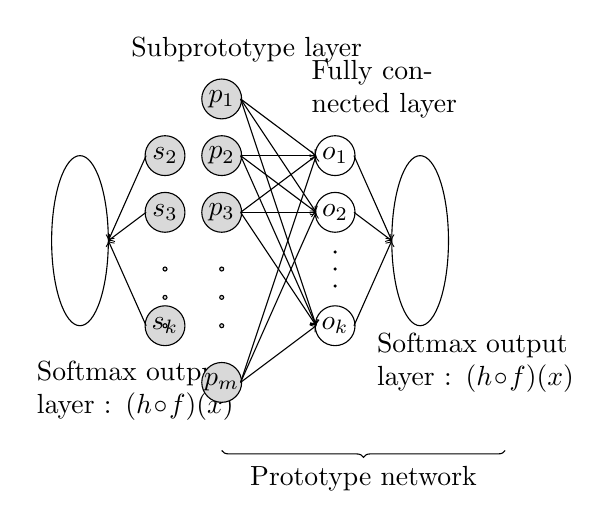
\begin{tikzpicture}[scale=0.72]
\coordinate (p1) at (0,0);
\coordinate (p2) at (0,2);
\coordinate (p3) at (0,3);
\coordinate (p4) at (0,4);
\coordinate (pn) at (0,5);
\coordinate (o1) at (2,1);
\coordinate (o2) at (2,2);
\coordinate (o3) at (2,3);
\coordinate (o4) at (2,4);

\coordinate (sp1) at (-1,1);
\coordinate (sp2) at (-1,2);
\coordinate (sp3) at (-1,3);
\coordinate (sp4) at (-1,4);
\coordinate (spn) at (-1,5);
\coordinate (so1) at (-3,1);
\coordinate (so2) at (-3,2);
\coordinate (so3) at (-3,3);
\coordinate (so4) at (-3,4);
% SUPER
\filldraw[fill=gray!30, draw=black] (sp1) circle (1em) node {$s_k$};
\filldraw[fill=gray!30, draw=black] (sp2) circle (0.1em);
\filldraw[fill=gray!30, draw=black] (-1,1.5) circle (0.1em);
\filldraw[fill=gray!30, draw=black] (-1,1) circle (0.1em);
\filldraw[fill=gray!30, draw=black] (sp3) circle (1em) node {$s_3$};
\filldraw[fill=gray!30, draw=black] (sp4) circle (1em) node {$s_2$};
%\filldraw[fill=gray!30, draw=black] (spn) circle (1em) node {$s_1$}  node[above, yshift=1em, text width=3cm, xshift=1em] {Superprototype layer};
\filldraw[fill=white, draw=black] (-2.5,2.5) ellipse (0.5 and 1.5) node[below,yshift=-4em, text width=2.5cm, xshift=2em] {Softmax output layer : $(h\circ f)(\bm{x})$};
  \foreach \j [evaluate=\j as \itext using int(\j)]in {1,3,4}
    {
      \path[->] (-1.333, \j) edge (-2, 2.5);
      \foreach \i [evaluate=\i as \itext using int(\i)] in {}
      {
        \draw[] () -- ();
      }
    }


% SUB
\filldraw[fill=gray!30, draw=black] (p1) circle (1em) node {$p_m$};
\filldraw[fill=gray!30, draw=black] (p2) circle (0.1em);
\filldraw[fill=gray!30, draw=black] (0,1.5) circle (0.1em);
\filldraw[fill=gray!30, draw=black] (0,1) circle (0.1em);
\filldraw[fill=gray!30, draw=black] (p3) circle (1em) node {$p_3$};
\filldraw[fill=gray!30, draw=black] (p4) circle (1em) node {$p_2$};
\filldraw[fill=gray!30, draw=black] (pn) circle (1em) node {$p_1$}  node[above, yshift=1em, text width=3cm, xshift=1em] {Subprototype layer};
\filldraw[fill=white, draw=black] (o1) circle (1em) node {$o_k$};
\filldraw[fill=gray!30, draw=black] (2,2) circle (0.05em);
\filldraw[fill=gray!30, draw=black] (2,2-0.3) circle (0.05em);
\filldraw[fill=gray!30, draw=black] (2,2+0.3) circle (0.05em);
\filldraw[fill=white, draw=black] (o3) circle (1em) node {$o_2$};
\filldraw[fill=white, draw=black] (o4) circle (1em)node {$o_1$} node [above,yshift=1em, text width=2cm, xshift=2em] {Fully connected layer};
 \foreach \i [evaluate=\i as \itext using int(\i)] in {0,3,4,5}
 {
    \foreach \j [evaluate=\j as \itext using int(\j)]in {1,3,4}
    {
      \path[->] (0.333, \i) edge (1.666666666666, \j);
    }
  }
\filldraw[fill=white, draw=black] (3.5,2.5) ellipse (0.5 and 1.5) node[below,yshift=-3em, text width=2.5cm, xshift=2em] {Softmax output layer : $(h\circ f)(\bm{x})$};
  \foreach \j [evaluate=\j as \itext using int(\j)]in {1,3,4}
    {
      \path[->] (2.333, \j) edge (3, 2.5);
    }
  \draw [decorate,decoration={brace,mirror}] (0,-1.2) -- (5,-1.2) node[midway,yshift=-10pt]{Prototype network};
\end{tikzpicture}}

    \caption{Architecture for a subprototype network\\ {\normalfont Gray nodes represent images encoded in latent space. {\color{red} Red} lines indicate the similarity between the input images and the subprototypes. In contrast, {\color{blue} blue} lines indicate the similarity between the superprototypes and subprototypes.}}
    \label{fig:hierarchical}
\end{figure}

We adjust the loss function to deal with the new layer. Error terms $R_1$ and $R_2$ force the subprototypes to be similar to at least one input data point and vice versa, as before. Two new terms, $R_3$ and $R_4$ are introduced to enforce similarity for a superprototype to at least one subprototype and vice versa. Thus, the superprototypes are connected to the subprototypes the same way the subprototypes are connected to the inputs. This highlights the hierarchicality of our network. The final loss term is:

\begin{align*}
    L((f,g,h),D) &= \lambda_{sub} E_{sub}(h_{\text{sup}} \circ f, D)\\ &+ \lambda_{sup} E_{sup}(h_{\text{sup}} \circ f, D) 
    + \lambda_R R(g \circ f,D)\\ &+ {\color{red}\lambda_1 R_1 + \lambda_2 R_2}  + {\color{blue}\lambda_3 R_3 + \lambda_4 R_4}
\end{align*}

Again, all $\lambda$'s are hyperparameters that can be used for weighting the various error terms.

By extending the loss function in this way, we ensure that superprototypes are not changed directly based on their relationship to the inputs, but indirectly through the subprototypes. The mechanics by which this is achieved are the same as the ones that make the subprototypes resemble the input ($R_1$ and $R_3$ are computed in the exact same way. The only difference are the inputs. The same holds for $R_2$ and $R_4$). In this way, there is a hierarchy between the subprototypes and superprototypes. Furthermore, by using the superprototypes to classify inputs and taking the cross-entropy error of this task into account in the loss function, we ensure that the superprototypes remain useful for the main task -- that is, classification. 

